\documentclass[11pt]{article}
\usepackage[utf8]{inputenc}
\usepackage{lmodern}
\usepackage{lipsum}
\usepackage[a4paper,width=160mm,top=25mm,bottom=25mm]{geometry}
\usepackage{multicol}
\setlength{\columnsep}{0.8cm}
\linespread{1.2}
\usepackage{gensymb}
\usepackage{stfloats}

\usepackage{array} % for defining a new column type
\usepackage{varwidth} %for the varwidth minipage environment


\def\blankpage{
  \clearpage
  \thispagestyle{empty}
  \addtocounter{page}{-1}
  \null
  \clearpage
}

\newenvironment{Figure}
  {\par\medskip\noindent\minipage{\linewidth}}
  {\endminipage\par\medskip}
  
\usepackage{titlesec}
\titleformat{\section}
  {\normalfont\sffamily\Huge\bfseries}
  {\thesection}{1em}{}
\titleformat{\subsection}
  {\normalfont\sffamily\large\bfseries}
  {\thesubsection}{1em}{}
\titleformat{\subsubsection}
  {\sffamily\bfseries}
  {\thesubsubsection}{1em}{}
  
\titlespacing{\section}{0pt}{1cm}{3cm}

\usepackage{tocloft}
\renewcommand{\cftsecfont}{\sffamily\bfseries}
\renewcommand{\cfttoctitlefont}{\sffamily\bfseries\Large}

\usepackage{graphicx}
\graphicspath{{Images/}}
\usepackage{caption}
\usepackage{subcaption}
\usepackage{array}
\usepackage{tabularx}
\usepackage{float}
\captionsetup[figure]{labelfont={bf,sf,small},textfont={sf,small}}

\usepackage[table,xcdraw]{xcolor}

\usepackage{fancyhdr}
\pagestyle{fancy}
\fancyhead{}
\fancyhead[C]{}
\fancyfoot{}
\fancyfoot[C]{\thepage}

\usepackage[backend=biber, style=numeric, citestyle=authoryear]{biblatex}

\addbibresource{references.bib}

\begin{document}
\newcolumntype{M}{>{\begin{varwidth}{4cm}}l<{\end{varwidth}}} %M is for Maximal column

    Annotating, analyzing and modeling of a video based personality trait corpus for mood primitives and likeability
    \pagebreak
    \thispagestyle{plain}
\begin{center}
    \Large
    \textsf{
        \textbf{
            Annotating, analyzing and modeling of a video based personality trait corpus for mood primitives and likeability
        }
    }
    
    \large
    \vspace{0.4cm}
    \textbf{Thomas Mol}
   
    \vspace{0.9cm}
    \Large
    \textsf{\textbf{Abstract}}
\end{center}

\hrule
\vspace{6pt}
Video based job interviews and resumes are increasing in popularity among organizations and corporations. They are a vital part in today's job candidate screening process and prove to be more cost efficient than previous types of interviews and resumes. These advancements make way for the automatic screening of job candidates by analyzing and modeling video based data-sets. To be more precise, the assessment of apparent personality traits and mood primitives give insight into the impressions a job candidate leaves on a job recruiter. In this thesis we describe a video based system that analyzes a video clip of a person and then produces personality trait and mood scores. On top of that, it predicts whether the person should be invited to a job interview or not. This thesis explores several types of classification models to make accurate predictions but also provide an explainable and interpretable model. The results show that the agreeableness, openness and conscientiousness dimensions have the most influence on the job interview prediction.


\vspace{6pt}
\hrule

\vfill

\begin{center}
    \Large
    \textsf{
        \textbf{Acknowledgments}
    }
\end{center}
I would like to thank Dr. Heysem Kaya and Prof. Dr. Albert Salah for their useful insight, feedback and knowledge throughout this project. I would also like to thank Bob Breemhaar for providing his annotations of the data-set.
    Video based job interviews and resumes are increasing in popularity among organizations and corporations. They are a vital part in today's job candidate screening process and prove to be more cost efficient than previous types of interviews and resumes. These advancements make way for the automatic screening of job candidates by analyzing and modeling video based data-sets. To be more precise, the assessment of apparent personality traits and mood primitives give insight into the impressions a job candidate leaves on a job recruiter. In this thesis we describe a video based system that analyzes a video clip of a person and then produces personality trait and mood scores. On top of that, it predicts whether the person should be invited to a job interview or not. This thesis explores several types of classification models to make accurate predictions but also provide an explainable and interpretable model. The results show that the agreeableness, openness and conscientiousness dimensions have the most influence on the job interview prediction.

\label{abstr}
    \pagebreak
    \tableofcontents\label{conte}
    \pagebreak
    
        \section{Introduction}\label{intro}
        \begin{multicols}{2}
        Affective computing and artificial intelligence are progressively becoming more popular and widely adopted by organizations (\cite{davenport2018artificial}, \cite{tao2005affective}). Affective computing systems intent to be responsive, interpret and recognize human affects, e.g., emotions. Many applications of such affective systems can be developed for educational tools, mental healthcare and much more. Furthermore, artificial intelligence and machine learning can be utilized in the development of affective systems. The performance capability of today's computer systems are becoming increasingly better to the point at which affective systems can be used in real-time. 

Another area where affective computing and machine learning methods can be applied is in the job candidate selection process. Job interviews are an essential part of the job candidate selection process for many corporations and organizations. Affective computing could help both the job seeker and the job recruiter. In this thesis we will explore a system that can predict whether an applicant should be invited to a job interview based on their perceived personality and mood. This system will be modeled based on video modality. Additionally, the system can help the job recruiter visualize biases in the selection process. The job seeker could also benefit from such a system as the system could show them what impression they give the recruiter and even suggest improvements to increase their chances to be invited to the job interview. 

Nevertheless, caution should be taken when developing and using such a system. It may seem like a game changer; a system that could automatically predict viable job candidates, especially when there is a staggering amount of candidates. However, supervised learning will be needed to create such a system. This means the system will rely on human based annotations for its supervision. As a result, the system will also learn the biases and stereotypes that annotators might have. For example, a younger age group is given higher overall job interview ratings compared to an older age group (\cite{morgeson2008review}). However, in actual job performance, the older workers are perceived to have better performance (\cite{truxillo2012perceptions}). Therefore, first impressions may not be a robust basis to determine actual job performance of a candidate.

In this thesis we will first discuss related literature on apparent personality traits, mood primitives and video resumes and job interview. Then, we will discuss our proposed methodology for our experiments which includes data annotation, feature extraction from video clips, feature normalization and lastly, classification and explainability models. We will also analyze the inter-rater agreement as we will have two annotators annotating our data-set. Next, we will report and discuss the results of the proposed experiments. After, we will look at the explainability analysis of the models. Lastly we will discuss our findings, shortcomings and describe future research than can be done regarding this research area. 

        \end{multicols}
        \pagebreak
        \twocolumn[
        \section{Related Literature}\label{theor}
        ]
        \subsection{Job Interviews \& Job Application Videos}
Many organizations and corporations utilize job interviews to select the most qualified person for an open position. Job interviews typically consist of a short meeting where the applicant is assessed based on their skills and experience but also on their personality, mood, energy and motivation during the interview. A study by Kraus and Kurtis (\citeyear{kraus1990creative}) shows that managers also base their decision heavily on their overall impression of the applicant. These dimensions are assessed to determine and predict if the applicant would be successful at the job they have applied for. Hiring an incompetent worker would not only mean the loss of salary but also the time it takes to search for a new candidate. A study by Dettmar (\citeyear{dettmar2004we}) shows that these implicit and explicit costs of hiring the wrong candidate combined could be as much as that of a years salary of that new hired worker. Despite this risk, job interviews prove to be a reliable method in the job candidate selection process (\cite{weekley1987reliability}). 

However, with the increase in use of online communication tools and online application processes job the approach for job interviews has changed as well. Many organizations choose to use online platforms to recruit new employees for open positions. A study in 2011 showed that 76\% of unemployed people search online for new jobs (\cite{faberman2016does}), which is an indication of how reliant organizations have become on online job recruitment. Research has been done to improve the online recruitment process by increasing market transparency and lower transaction cost with the use of semantic web technologies (\cite{bizer2005impact}). Further, video resumes have become increasingly popular as a result of the increase of use of online communication platforms. Studies show that video resumes are mostly made by a young demographic who are looking for a junior position (\cite{nguyen2016hirability}). In addition to online video resumes, a new type of online job interviewing has also emerged which is called asynchronous video interviews (\cite{torres2017asynchronous}). This type of interviewing involves an applicant who sends a video recording of them answering interview questions (\cite{toldi2011jobapplicants}). On the other hand, synchronous video interviewing are held on platforms like Skype, Microsoft Teams and other video conference software. These new methods of interviewing can decrease costs as they prove to be more time-efficient (\cite{weber2012your}).

\subsection{Analyzing Personality Traits}
The assessment of personality traits is equally important when analyzing and determining which candidate is the most suitable for the position (\cite{kinsman2005hiring}). However, assessing a person's personality can be a rather difficult task. Therefore we must first understand how personality is defined and how to analyze it. 

In psychology, the characterization of someone's personality is based on long-term behavior. Personalities have sophisticated structures and are constructed of many different aspects such as habits and the way people think or feel. Therefore it can be difficult to analyze, measure and categories personalities to divide humans into different personality types. Instead, psychology now mainly focuses on personality traits, where the OCEAN (or CANOE) Big Five personality trait model developed by Paul Costa and Robert R. McCrae (\cite{costa1992neo}) is most widely accepted. These traits are; Openness to experience, Conscientiousness, Extraversion, Agreeableness and lastly, Neuroticism. 

The first factor of the 5 factor personality trait model is Openness to experience. People who score high in this factor generally are imaginative and care more about aesthetics, ideas and values (\cite{mccrae1993openness}). The Conscientiousness factor is related to how well-organized and persistent a person is. People with high conscientiousness are considered caring, dependable and organized (\cite{widiger2017oxford}). The traits underlying the Extraversion dimension are related to sociability and activity. Extraverted people are more talkative, adventurous and sociable while introverted people tend to be more silent, cautious and focused on their inner state of mind(\cite{widiger2017oxford}). Agreeableness is a dimension of interpersonal behavior. People with high scores on agreeableness are cooperative, good natured and are seen as friendly (\cite{graziano1997agreeableness}). Lastly, the Neuroticism dimension represents a person's tendency to experience emotional anxiety (\cite{widiger2017oxford}). The dimension can also be described as someone's emotional stability. People with high neuroticism are more anxious and nervous and tend to worry more while people with low scores are more calm and composed. 

Several works have used this model to analyze human behavior like \textcite{quercia2011our} who analyzed relationships with different types of Twitter users. Or \textcite{allbeck2008creating}, who used the OCEAN model to map personalities to crowd simulations in order to improve the realism of their simulations. 

\subsubsection{Apparent Personality Analysis}

Another approach to apply the five factor model is to analyze and annotate the apparent personality traits (\cite{junior2018first}, \cite{chen2016overcoming}), rather than the actual personality traits. In this process an annotator annotates the impression a subject leaves rather than the actual personality. This is easier as the annotator relies on external evaluations without any direct involvement of the subject. 

Several studies have shows that the modeling of apparent personality traits is possible from different modalities like text (\cite{gievska2014impact}, \cite{alam2013personality}), speech (\cite{valente2012annotation}, \cite{madzlan2014towards}) and also video based (\cite{junior2018first}, \cite{qin2016modern}, \cite{escalante2020modeling}e). On top of that, research has been on modeling job interview decisions based on apparent personality traits from different modalities (\cite{kaya2017multi}, \cite{kaya2018multimodal}, \cite{yu2019multimodal}).

\subsection{Mood Primitives \& Likeability}
Another dimension that can be used to classify a person's behavior is to assess their mood or emotions over a short period of time. While the terms emotion and mood seem to be used interchangeably, they are in fact different. In psychology, an emotion is seen as a immediate reaction to a stimulus, while a mood lasts for a longer period (\cite{bower2000affectmemory}). For example, someone can be in positive mood throughout the day but still have a negative emotional reaction to a stimulus like a bad smell, or being insulted (\cite{matlin2012cognition}). Additionally, this makes is more difficult to identify and specify the cause of someone's mood as there is no direct cause like in a emotional reaction (\cite{desmet2016mood}).

In order to simplify the classification of a subject's mood, emotion classification can be used. Instead of trying to determine someone's mood over a short period, the emotions can be used as an indicator or their mood. To do this, a base set of emotions is needed to start classifying a subject's mood. The six basic emotions developed by Paul Ekman in 1992 are widely regarded as the standard to identify emotions (\cite{ekman1992argument}). Figure \ref{fig:basicemotion} illustrates the emotions as described by Ekman. Ekman found that there are nine distinct characteristics that distinguish the basic emotions, for example, the physiological response, the duration and their quick onset. He also found that cultural background had no impact in the identification of emotion. Meaning that the six basic emotion can be used across different cultures to classify emotions. The six emotion that Ekman identified as basic are; anger, happiness, surprise, disgust, sadness and fear (\cite{ekman1992argument}). 

\begin{figure}[h]
  \centering
  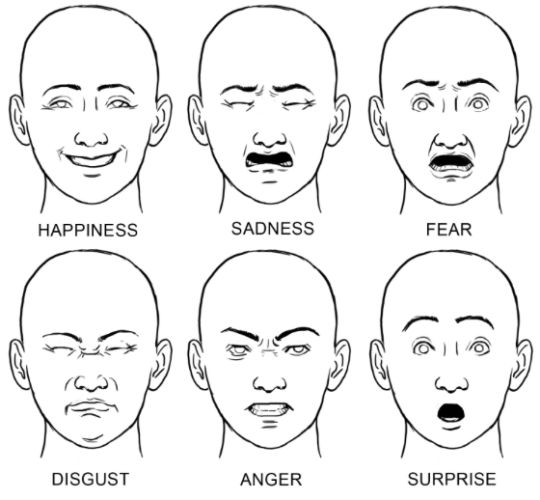
\includegraphics[width=\columnwidth]{Images/ekman_six_emotion.png}
  \caption{The 6 basic emotions as proposed by Ekman.}
  \label{fig:basicemotion}
\end{figure}

Research has also indicated that mood can be defined as a dimensional model with two dimensions: valence and arousal. This model was first proposed by Russel in 1980 (\cite{russell1980circumplex}), and is known as the circumplex model of affect. In this model arousal can be seen as the amount of energy a person shows. This dimension ranges from a deactivated state, described as sleepiness, to an activated state, which can be described as aroused. The valence dimension refers to the pleasantness or unpleasantness. This dimension typically ranges from a state of misery to a state of pleasure. Combining these two dimension creates four quadrants with four basic moods; angry, happy, sad and relaxed. Figure \ref{fig:circumplexrussel} shows the circumplex model and indicates where the basic moods would be posistioned on this model. 

\begin{figure}[h]
  \centering
  \includesvg[width=\columnwidth]{Images/russell_dimensions.svg}
  \caption{The circumplex model of affect as proposed by Russel.}
  \label{fig:circumplexrussel}
\end{figure}


        \pagebreak
        \twocolumn[
        \section{Methodology}\label{methd}
        ]
        
Our proposed method analyzes a video clip containing one person. The output is an estimate of the interview invitation variable, the big five OCEAN personality traits, the two mood primitives valence and arousal and lastly, the likeability variable. Only video features are used in our proposed method. This section will describe the main stages of our method, starting with describing our data-set and the process of annotating this data. Then the feature extraction and normalization processes are defined. Lastly, the classification methods are described. Figure \ref{fig:proposedmethod} shows the pipeline of our proposed method.

\begin{figure*}[h]
  \centering
  \includesvg[width=\textwidth]{Images/method_pipeline.svg}
  \caption{Flowchart of the proposed methodology.}
  \label{fig:proposedmethod}
\end{figure*}

\subsection{The Data Set}
\label{subsection:dataset}

For modeling and experimenting we relied on a publicly available data-set which contains 10,000 video clips with audio with an average duration of 15 seconds\footnote{The data-set can be found on http://chalearnlap.cvc.uab.es/dataset/24/description/}. The clips are collected from over 3000 videos available on YouTube. Figure \ref{fig:ssvideoclip} shows screenshots from four samples taken from the video clip data-set. The videos are annotated with the use of Amazon Mechanical Turk for apparent personality traits. These are the 5 OCEAN personality traits variables. Annotators saw a pair of video clips and were asked to assign an attribute to one of the videos with the option to not assign an attribute at all. These attributes are words describing the 5 OCEAN personality traits. 

Furthermore, the videos are annotated for an additional variable, which is the interview variable. This variable measures whether a candidate should be invited for a job interview or not. Additionally these videos are annotated for ethnicity groups, age groups and gender (\cite{escalante2018explaining}). From this data-set of 10,000 videos the first 960 were selected for experimenting and further annotations of three more variables, namely, the valence, arousal and likeability variables. 


\begin{figure*}[h]
  \centering
  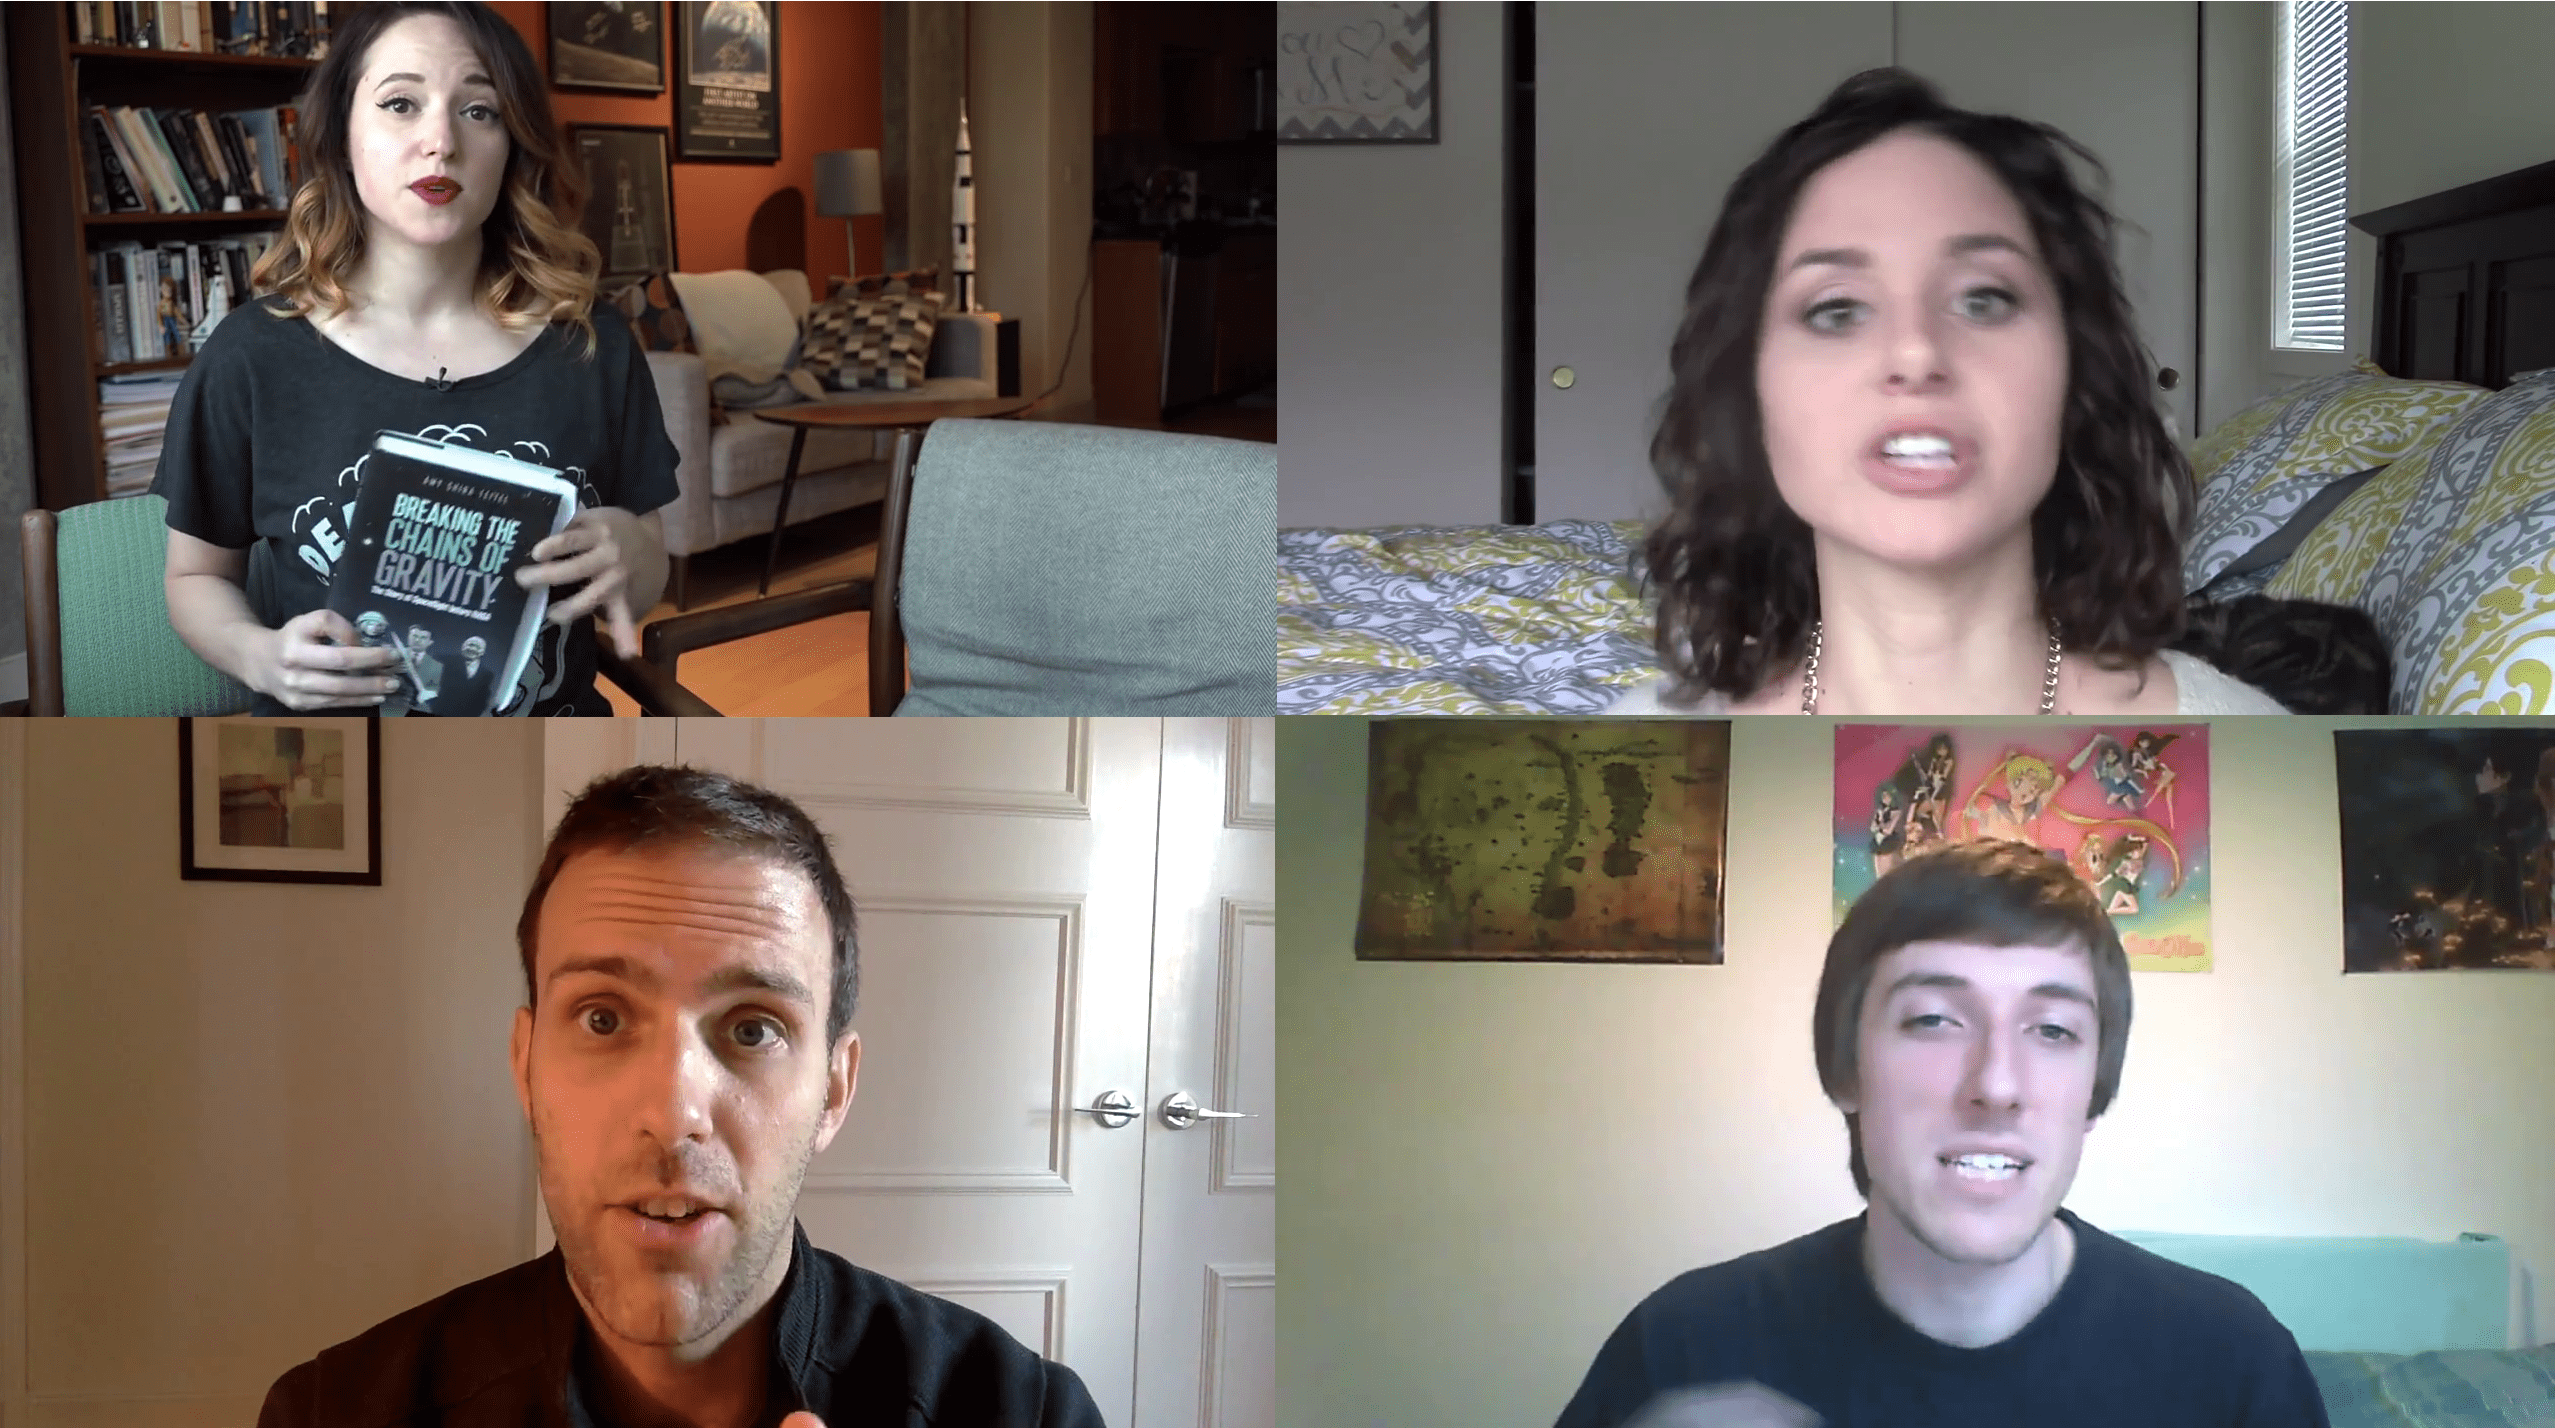
\includegraphics[width=0.8\textwidth]{Images/sample_video_clips-min.png}
  \caption{Screenshots from four samples of the video clip data-set.}
  \label{fig:ssvideoclip}
\end{figure*}


\subsection{Annotating Data}
\label{subsection:annotatingdata}
The selected 960 video clips were annotated additionally for mood primitives, likeability and a variable describing the presence of background music. The mood primitives, valence and arousal, and likeability were annotated with an ordinal scale with 3 classes. An annotation of class 1 means the variable scored low or negatively, class 2 is the neutral case, and class 3 means the variable scored high or positively. Initially the scale was set with 5 classes, however annotations with class 1 or class 5 were scarce so a smaller scale was chosen to improve the accuracy of the models. 

Two annotators annotated the same 960 video clips for these 4 dimensions. After which, the annotations were merged to create two additional data-sets. One data-set used the minimum of the two annotation, while the second one used the maximum of the two annotations. As a result, there were now 4 sets of annotations available to use and model classifiers with.

To measure the inter-rater reliability between the two annotators the Cohen's kappa coefficient was calculated. This coefficient is considered more robust as it takes into account the occurrence of an agreement by chance. The resulting coefficient will determine whether the agreement is accidental or not. Table \ref{tab:cohenkappa} shows the results of the Cohen's kappa calculations. The observed agreement (po) is the number of agreements divided by the total of number items. The random agreement (pe) is the probability that the annotators agreed on either of the possible annotations. Using the observed and random agreement the Cohen's kappa can be calculated. The coefficient ranges from 0 to 1 and can be interpreted as shown in table \ref{tab:cohenkappainterpret}.

\begin{table*}[]
\begin{tabular}{|l|l|r|r|r|P{1.3cm}|P{2cm}|P{2cm}|}
\hline
\rowcolor{Gray}
\textbf{Dimension} & \textbf{Weight} & \multicolumn{1}{l|}{\textbf{po}} & \multicolumn{1}{l|}{\textbf{pe}} & \multicolumn{1}{l|}{\textbf{Kappa}} & \multicolumn{1}{l|}{\textbf{Kappa Error}} & \textbf{Agreement} & \textbf{Null hypothesis} \\ \hline
\multirow{3}{*}{\textbf{Arousal}} & Unweighted & 0.6229 & 0.4077 & 0.3634 & 0.0264 & Fair & Rejected \\ \cline{2-8} 
 & Linear & 0.8073 & 0.6713 & 0.4138 & 0.0387 & Moderate & Rejected \\ \cline{2-8} 
 & Quadratic & 0.8995 & 0.8031 & 0.4896 & 0.0493 & Moderate & Rejected \\ \hline
\multirow{3}{*}{\textbf{Valence}} & Unweighted & 0.7177 & 0.5046 & 0.4302 & 0.0293 & Moderate & Rejected \\ \cline{2-8} 
 & Linear & 0.8573 & 0.7371 & 0.4571 & 0.0429 & Moderate & Rejected \\ \cline{2-8} 
 & Quadratic & 0.9271 & 0.8534 & 0.5027 & 0.0572 & Moderate & Rejected \\ \hline
\multirow{3}{*}{\textbf{Likeability}} & Unweighted & 0.5812 & 0.4230 & 0.2743 & 0.0276 & Fair & Rejected \\ \cline{2-8} 
 & Linear & 0.7818 & 0.6704 & 0.3380 & 0.0404 & Fair & Rejected \\ \cline{2-8} 
 & Quadratic & 0.8820 & 0.7941 & 0.4272 & 0.0506 & Moderate & Rejected \\ \hline
\end{tabular}
\caption{Inter rater agreement results. po: observed agreement, pe: random agreement, Kappa: Cohen's Kappa.}
\label{tab:cohenkappa}
\end{table*}

\begin{table}[]
\begin{tabular}{|P{2cm}|P{4cm}|}
\hline
\rowcolor{Gray}
Cohen's Kappa & Agreement \\ \hline
0 & Agreement equivalent to chance \\ \hline
0.10 - 0.20 & Slight \\ \hline
0.21 - 0.40 & Fair \\ \hline
0.41 - 0.60 & Moderate \\ \hline
0.61 - 0.80 & Substantial \\ \hline
0.81 - 0.99 & Near perfect \\ \hline
1 & Perfect \\ \hline
\end{tabular}
\caption{Cohen's kappa agreement interpretation.}
\label{tab:cohenkappainterpret}
\end{table}

Since Cohen's kappa takes into account the disagreement but not the degree of disagreement a modified version of Cohen's kappa can be used which is the weighted Cohen's kappa (\cite{cohen1968weighted}). This can be applied well if an ordinal scale is used for the ratings. Since the annotations of the data-set use an ordinal scale, the weighted Cohen's kappa can be applied. The weighted kappa is calculated with the use of a table containing weights which measure the degree of disagreement. This can be linear or quadratic. Table \ref{tab:cohenkappa} shows the results of the weighted Cohen's kappa alongside the unweighted versions. 

Overall, every dimension shows a moderate agreement when quadratic weighting is applied. Further, for every dimension and weight the null hypothesis is rejected, where the null hypothesis is that the observed agreement is accidental. Therefore it is safe to say the inter-rater reliability is higher than chance level. The data was then split up in a train set of 660 video clips and a test set of 300 video clips to be used for model training, optimization and testing. 

\subsection{Video Feature Extraction}\label{subsection:featureextraction}
To train our models we use video features that are extracted from the 15 second YouTube clips provided by the ChaLearn Competition. The features are facial features which are extracted over the entire video clip. These features are summarized by functionals. First, the faces were detected and then aligned using the Supervised Descent Method (\cite{xiong2013supervised}). Every detected face is rotated using the roll angle which is estimated from the eye corners. Also, there are 49 landmarks located on each face to which a 20\% margin is applied to corp the image to a size of 64 x 64 pixels. Image-level features are extracted from a convolutional neural network which was trained for emotion recognition. This network is a pre-trained VGG-Face network (\cite{kaya2017video}), which is optimized for large data-sets. The final layer of the network was changed to a 7-dimensional emotion recognition layer. The resulting network was then fine-tunes using the FER-2013 data-set (\cite{goodfellow2015challenges}), which contains over 30,000 images. The final trained network has 37 layers from which the 33rd response was used. This descriptor has 4096 dimensions which were then summarized using four statistical functions. Those functions were the mean, standard deviation, slope and offset from a linear polynomial.

\subsection{Feature Normalization}
\label{subsection:normalization}
Z normalization transforms the input vector into a vector where the mean is 0 or very close to 0 while the standard deviation is close to 1. The number for a single data point of the computed output vector can also be called the z-score. This score essentially is the number of standard deviations a vector is away from the mean. It can indicate how familiar a data point is relative to the others. 

\begin{figure*}[h]
  \centering
  \includesvg[width=\textwidth]{Images/featurenormalization_pipeline.svg}
  \caption{Feature normalization pipeline}
  \label{fig:normpipeline}
\end{figure*}

While Z normalization is applied at feature level L2 normalization is applied at feature vector level. L2 normalization is applied at each row of the feature set so that if the values are squared and then summed, they add up to exactly 1. 

Figure \ref{fig:normpipeline} shows the flowchart of the normalization steps that were applied at feature and vector level. 



\subsection{Classification Algorithms}
\label{subsection:classificaiton}
Several types of models were used for classification from the extracted video features. These models include:
\begin{enumerate}
\item Extreme Learning Machines (ELM)
\item Support Vector Machines (SVM)
\item Decision Trees (DT)
\item Ridge Classification
\end{enumerate}
In the first stage we use the ELM and SVM classifiers, while in the second stage we use the predictions of the ELM classifier to train a decision tree and linear model. The second stage classifications will give an indication of the feature importance and contribute to the explainability of our classification models. 

Originally proposed by Huang in 2004 (\cite{huang2004extreme}), the learning algorithm for Extreme Learning Machine uses single-hidden layer feedforward neural networks (SLFN). It chooses the nodes randomly and analytically determines the the output weights for the neural network. As a result, the training speed of this algorithm is noticeably fast. The technical details of the classifiers can be found in \cite{huang2004extreme} and \cite{huang2006extreme}. We use a linear kernel which has a regularization coefficient. We optimize this coefficient during training and with threefold subject independent cross-validation of the training set. 

Just like ELM, the SVM algorithm is used for regression and classification. SVMs is a supervised learning method which is effective when the number of features is high or even higher than the number of samples. The algorithm finds the hyperplane in a dimensional space of size N, where N is the number of features. It then uses the hyperplane to classify the data-points. To obtain the most accurate model the algorithm finds the hyperplane where the margins of the hyperplane are the largest. Just like the ELM algorithm a linear kernel is used and a regularization coefficient is optimized. 

The models that are trained using the ELM and SVM algorithms will create a set of predictions of the personality trait, mood and likeability dimensions. The predictions of the ELM classifier will be used in the second stage of our classification. During this stage, the predictions are stacked to a Decision Tree classifier as high level features. The DT classifier is trained using the predictions and the interview invitation variable as labels. Then, the trained DT can be visualized which contributes to the explainability and interpretability of our classification model.

Lastly, the same prediction data set to train the Decision Tree classifier is used to train a linear model. We will be using the Ridge Classifier which converts the target values to -1 and 1. Then, the model treats the problem as a regression problem. The trained model will provide us with the coefficient of the features of the decision function. In other words, the feature importance can be derived from these models which will show us what feature is the most or least important for determining the class.



        \pagebreak
        \twocolumn[
        \section{Experiment Results}\label{resul}
        ]
        This section will provide, analyze and discuss the results of the annotations and of the experiments done with the data-set. First, general statistics will be provided regarding the mood and likeability annotations. Then the new annotations in conjunction with the interview variable will be analyzed to identify any statistical relationship. Next, we will provide the results of the experiments. The performance of the models created during the experiments will be expressed in their Unweighted Average Recall or UAR. The UAR is the mean of the recall scores of each class. The recall is the ratio between the number of true positives and false negatives. If all predictions would be correctly classified the UAR would be 1. The UAR metric  is a better indication of prediction capacity than precision accuracy as our data-set is imbalanced. The UAR does not favor the majority class and is therefore a better indicator of the prediction capabilities of our models.
\break

\subsection{Annotation Analysis}
As described in the methodology, 960 video clips of the data-set were annotated for the Big Five personality traits, two mood primitives (valence and arousal), likeability, background music and the interview variable. The personality and interview dimensions were annotated using Amazon Mechanical Turk. All dimensions, with the exception of background music, were annotated for apparent presence or absence. The interview variable indicates whether the annotator would invite the subject to an interview or not. Table \ref{tab:personcount} and table \ref{tab:goldcount} show the number of annotations for each class and dimension. 

The apparent personality trait and interview dimensions were post-processed to create cardinal scores for each video clip (\cite{escalante2018explaining}). These scores were also binarized by taking the mean of each dimension and assigning a 2 if the score was equal or higher than the mean and assigning a 1 if the score was lower than the mean. Table \ref{tab:personcount} shows the number of annotations based on the binarized data-set. 

\begin{table}[h]
\begin{tabular}{|r|r|r|r|}
\hline
\rowcolor[HTML]{C0C0C0} 
\multicolumn{1}{|l|}{\cellcolor[HTML]{C0C0C0}Class} &
  \multicolumn{1}{l|}{\cellcolor[HTML]{C0C0C0}Arousal} &
  \multicolumn{1}{l|}{\cellcolor[HTML]{C0C0C0}Valence} &
  \multicolumn{1}{l|}{\cellcolor[HTML]{C0C0C0}Likeability} \\ \hline
1                           & 77  & 46  & 99  \\
2                           & 364 & 707 & 505 \\
3                           & 519 & 207 & 356 \\ \hline
\multicolumn{1}{|l|}{Total} & 960 & 960 & 960 \\ \hline
\end{tabular}
\caption{Number of annotations (self) per class of the mood primitive and likeability dimensions}
\label{tab:selfcount}
\end{table}

\begin{table}[h]
\begin{tabular}{|r|r|r|r|}
\hline
\rowcolor[HTML]{C0C0C0} 
\multicolumn{1}{|l|}{\cellcolor[HTML]{C0C0C0}Class} &
  \multicolumn{1}{l|}{\cellcolor[HTML]{C0C0C0}Arousal} &
  \multicolumn{1}{l|}{\cellcolor[HTML]{C0C0C0}Valence} &
  \multicolumn{1}{l|}{\cellcolor[HTML]{C0C0C0}Likeability} \\ \hline
1                           & 108 & 82  & 197 \\
2                           & 593 & 705 & 602 \\
3                           & 259 & 173 & 161 \\ \hline
\multicolumn{1}{|l|}{Total} & 960 & 960 & 960 \\ \hline
\end{tabular}
\caption{Number of annotations (gold min) per class of the mood primitive and likeability dimensions}
\label{tab:goldcount}
\end{table}

\begin{table*}[th]
\begin{tabular}{|r|r|r|r|r|r|r|}
\hline
\rowcolor[HTML]{C0C0C0} Class &
  \multicolumn{1}{l|}{Openness} &
  \multicolumn{1}{l|}{Conscientiousness} &
  \multicolumn{1}{l|}{Extraversion} &
  \multicolumn{1}{l|}{Agreeableness} &
  \multicolumn{1}{l|}{Neuroticism} &
  \multicolumn{1}{c|}{Interview Invitation} \\ \hline
1     & 528 & 458 & 443 & 437 & 441 & 426 \\ \hline
2     & 432 & 502 & 517 & 523 & 519 & 534 \\ \hline
Total & 960 & 960 & 960 & 960 & 960 & 960 \\ \hline
\end{tabular}
\caption{Number of annotations per class of apparent personality trait and interview invitation dimensions}
\label{tab:personcount}
\end{table*}

\subsection{Statistical Relationships}

Some interesting statistical experiments can be done regarding the statistical relationship of the mood primitives and likeability dimensions and the interview invitation. For these experiments we will use the cardinal values of the interview variable. Three box-plots are created using this data and can be seen in figure \ref{fig:boxplotval}, figure \ref{fig:boxplotaro} and figure \ref{fig:boxplotlike}. For these box-plots the y-axis indicates the cardinal interview invitation variable, where a higher score means they would be more likely to be invited for an interview. The x-axis indicate the three classes of the arousal, valence or likeability dimensions. The orange horizontal line in the box-plots indicate the mean. As the plots show, there is a upwards trend in the mean of all three box-plots. Meaning that if the subject is classified in the higher class, they would be more likely to be invited to a job interview.

\begin{figure}[h]
  \centering
  \includesvg[width=\columnwidth]{Images/boxplot_valence_interview.svg}
  \caption{Box-plot of the valence classes and interview invitation variable}
  \label{fig:boxplotval}
\end{figure}

\begin{figure}[h]
  \centering
  \includesvg[width=\columnwidth]{Images/boxplot_arousal_interview.svg}
  \caption{Box-plot of the arousal classes and interview invitation variable}
  \label{fig:boxplotaro}
\end{figure}

\begin{figure}[h]
  \centering
  \includesvg[width=\columnwidth]{Images/boxplot_likeability_interview.svg}
  \caption{Box-plot of the likeability classes and interview invitation variable}
  \label{fig:boxplotlike}
\end{figure}

However, to see if there is a correlation between the interview variable and mood and likeability variables we must look at the Spearman's Rank-Order Correlation coefficient. This coefficient can used to calculate correlation for ordinal categorical variables. To calculate this coefficient we will be using the binarized data-set of the interview variable. The coefficient is calculated as follows: \(\rho = \frac{cov(x,y)}{\sigma_x \sigma_y}\), where \(cov(x,y)\) is the covariance of the variables and \(\rho\) is the Pearson correlation coefficient. Table \ref{tab:spearman} shows the correlation and p value between the three dimensions and the binarized interview variable. The results show a low p value for all dimensions, with every p value being close to 0. This means that the null hypothesis should be rejected, where the null hypothesis is that two sets of data are uncorrelated. By rejected the null hypothesis we can conclude that the sets of data are not uncorrelated, however it does not prove that they are correlated. If we look at table \ref{tab:spearman} we can see that the correlation values are between 0.2 and 0.4. For the arousal dimension this means that the strength of the correlation is small, while for the valence and likeability dimensions there is medium strong correlation. A perfect correlation would be indicated with a value of 1 or -1 (for a negative correlation). Typically, a correlation is considered strong if the value is higher than 0.7 or lower than -0.7. 

\begin{table}[h]
\begin{tabular}{|l|r|r|r|}
\hline
\rowcolor[HTML]{C0C0C0} 
 & \multicolumn{1}{l|}{\cellcolor[HTML]{C0C0C0}Arousal} & \multicolumn{1}{l|}{\cellcolor[HTML]{C0C0C0}Valence} & \multicolumn{1}{l|}{\cellcolor[HTML]{C0C0C0}Likeability} \\ \hline
Correlation & 0.296 & 0.204 & 0.395 \\ \hline
P Value & 6.51E-21 & 1.76E-10 & 3.09E-37 \\ \hline
\end{tabular}
\caption{Results of the Spearman Rank Correlation coefficient calculations}
\label{tab:spearman}
\end{table}

\subsection{Mood and Likeability Model Experiments}
In this section we will discuss the performance of the models that are trained using the mood and likeability dimensions and the extracted video features. As stated in the methodology the data-set was split into a training set of 660 rows and a test set of 300 rows. Both the self annotation and the gold standard annotations were used for training the classifiers. Models using ELMs and SVMs wer

\begin{table*}[h]
\begin{tabular}{|l|l|r|r|r|r|r|r|}
\hline
\rowcolor[HTML]{C0C0C0} 
\textbf{Weighted} & \textbf{Normalization} & \multicolumn{1}{l|}{\cellcolor[HTML]{C0C0C0}\textbf{self\_arousal}} & \multicolumn{1}{l|}{\cellcolor[HTML]{C0C0C0}\textbf{gold\_arousal}} & \multicolumn{1}{l|}{\cellcolor[HTML]{C0C0C0}\textbf{self\_valence}} & \multicolumn{1}{l|}{\cellcolor[HTML]{C0C0C0}\textbf{gold\_valence}} & \multicolumn{1}{l|}{\cellcolor[HTML]{C0C0C0}\textbf{self\_like}} & \multicolumn{1}{l|}{\cellcolor[HTML]{C0C0C0}\textbf{gold\_like}} \\ \hline
\textbf{No} & \textbf{NN} & \cellcolor[HTML]{FFE2E2}39.79\% & \cellcolor[HTML]{FFAEAE}42.67\% & \cellcolor[HTML]{FFF9E7}47.91\% & \cellcolor[HTML]{FFF9E9}47.78\% & \cellcolor[HTML]{FFFFFF}38.47\% & \cellcolor[HTML]{D1EDDF}42.61\% \\ \hline
\textbf{No} & \textbf{ZN} & \cellcolor[HTML]{FF9B9B}43.76\% & \cellcolor[HTML]{FF2E2E}49.88\% & \cellcolor[HTML]{FFF4D5}49.11\% & \cellcolor[HTML]{FFFFFF}46.21\% & \cellcolor[HTML]{6DC499}51.56\% & \cellcolor[HTML]{88CFAD}49.11\% \\ \hline
\textbf{No} & \textbf{L2} & \cellcolor[HTML]{FFE1E1}39.80\% & \cellcolor[HTML]{FFB2B2}42.49\% & \cellcolor[HTML]{FFFAEC}47.53\% & \cellcolor[HTML]{FFFCF1}47.19\% & \cellcolor[HTML]{F0F9F5}39.84\% & \cellcolor[HTML]{CAEADA}43.25\% \\ \hline
\textbf{No} & \textbf{ZN+L2} & \cellcolor[HTML]{FFE4E4}39.68\% & \cellcolor[HTML]{FF5656}47.63\% & \cellcolor[HTML]{FFF1C9}49.95\% & \cellcolor[HTML]{FFFEF9}46.64\% & \cellcolor[HTML]{8DD1B0}48.68\% & \cellcolor[HTML]{7FCBA6}49.98\% \\ \hline
\textbf{Yes} & \textbf{NN} & \cellcolor[HTML]{FFC1C1}41.60\% & \cellcolor[HTML]{FF5F5F}47.15\% & \cellcolor[HTML]{FFF5D7}49.00\% & \cellcolor[HTML]{FFE8A8}52.25\% & \cellcolor[HTML]{70C59B}51.33\% & \cellcolor[HTML]{5CBE8E}53.04\% \\ \hline
\textbf{Yes} & \textbf{ZN} & \cellcolor[HTML]{FF8383}\textbf{45.13\%} & \cellcolor[HTML]{FF0000}\textbf{52.46\%} & \cellcolor[HTML]{FFE9AD}\textbf{51.92\%} & \cellcolor[HTML]{FFDA73}55.92\% & \cellcolor[HTML]{5BBD8D}\textbf{53.19\%} & \cellcolor[HTML]{86CEAB}49.32\% \\ \hline
\textbf{Yes} & \textbf{L2} & \cellcolor[HTML]{FFFFFF}38.11\% & \cellcolor[HTML]{FF1919}51.08\% & \cellcolor[HTML]{FFF3D2}49.36\% & \cellcolor[HTML]{FFD666}\textbf{56.77\%} & \cellcolor[HTML]{66C195}52.18\% & \cellcolor[HTML]{57BB8A}\textbf{53.49\%} \\ \hline
\textbf{Yes} & \textbf{ZN+L2} & \cellcolor[HTML]{FF9898}43.91\% & \cellcolor[HTML]{FF0202}52.37\% & \cellcolor[HTML]{FFF1C8}50.05\% & \cellcolor[HTML]{FFE8A6}52.38\% & \cellcolor[HTML]{5CBD8E}53.08\% & \cellcolor[HTML]{7BCAA3}50.35\% \\ \hline
\end{tabular}
\caption{Linear Kernel Extreme Learning Machine model performance results expressed in UAR}
\label{tab:lkelm}
\end{table*}

\subsection{Personality Trait experiments}
        \pagebreak
        \onecolumn
        \section{Conclusion \& Discussion}\label{concl}
        Video based job interviews and resumes are becoming increasingly popular methods for organizations to adopt in their hiring process. Automatic personality trait and mood could vastly accelerate and support this process. As the literature illustrates, personality traits and mood are important factors that influence the decision to invite an applicant to an interview. Creating such automated systems can only be done however, if the trained models are highly accurate and do not show bias. Therefore, the experiments done in this thesis are to compare and improve classification models using extracted video features which can lead to better automated job screening systems.

Several experiments have been done using our data-set, ranging from classification of dimensions to creating explainable models like decision trees. The ELM algorithm has proven to be an accurate to model mood and likeability dimensions from a set of video features. With UAR scores of up to 57\%, the performance was considerably above the chance level of 33\%. Further, the results show ELM models have also proven to be more accurate than the widely used support vector machine algorithm. Also, a moderate correlation has been found between the interview invitation variable and the mood and likeability dimensions. Despite this correlation, the decision tree model and feature importance experiment show that valence and arousal play a minor role in the prediction of the interview invitation variable. The personality traits, especially openness, agreeableness and conscientiousness show to be more important factors in predicting the interview invitation variable. The resulting decision tree could be used to help job recruiter in the job screening process. However, it is strongly recommended that more modalities and dimensions should be explored before such a classification system should be used in the wild. The experiments done in this thesis only utilized video features from the video clips in the data-set. However, video resumes obviously also include acoustics which should be used in combination of video features to create more accurate models. 

A great deal of future research can be done with the data-set that was used for this thesis. For example, the data-set is also annotated for ethnicity, age groups, gender and background music. These variables are annotated using a categorical scale. Therefore the data-set could be split into different categories regarding these dimensions which could result in interesting new decision trees and model results. It could also expose biases towards the different categories of these dimensions from the annotators, or expose a bias a job recruiter might have. Also, in this thesis only the video features are used to train the models. Also, for the modeling stage only 960 samples were used of the available 10,000 video clips. If a larger sample size, if not all video clips, would also be annotated for the mood and likeability dimensions, the performance of the classifications model could be improved. This could also lead to better explainability models. The bias of the annotators regarding ethnicity, age groups and gender was also not explored. Further analysis of this data could expose biases and therefore also illustrate biases in the classification models. 
        \pagebreak
    \thispagestyle{plain}
    \printbibliography[heading=bibintoc,title={References}]
    \pagebreak
    
    
\end{document}
